\documentclass[letterpaper]{article}
\usepackage[margin=1in]{geometry}
\usepackage[utf8]{inputenc}
\usepackage{textcomp}
\usepackage{amssymb}
\usepackage{natbib}
\usepackage{graphicx}
\usepackage{gensymb}
\usepackage{amsthm, amsmath, mathtools}
\usepackage[dvipsnames]{xcolor}
\usepackage{enumerate}
\usepackage{mdframed}
\usepackage[most]{tcolorbox}
\usepackage{csquotes}
% https://tex.stackexchange.com/questions/13506/how-to-continue-the-framed-text-box-on-multiple-pages

\tcbuselibrary{theorems}

\newcommand{\R}{\mathbb{R}}
\newcommand{\Z}{\mathbb{Z}}
\newcommand{\N}{\mathbb{N}}
\newcommand{\Q}{\mathbb{Q}}
\newcommand{\C}{\mathbb{C}}
\newcommand{\code}[1]{\texttt{#1}}
\newcommand{\mdiamond}{$\diamondsuit$}
\newcommand{\PowerSet}{\mathcal{P}}
\newcommand{\Mod}[1]{\ (\mathrm{mod}\ #1)}
\DeclareMathOperator{\lcm}{lcm}

%\newtheorem*{theorem}{Theorem}
%\newtheorem*{definition}{Definition}
%\newtheorem*{corollary}{Corollary}
%\newtheorem*{lemma}{Lemma}
\newtheorem*{proposition}{Proposition}


\newtcbtheorem[number within=section]{theorem}{Theorem}
{colback=green!5,colframe=green!35!black,fonttitle=\bfseries}{th}

\newtcbtheorem[number within=section]{definition}{Definition}
{colback=blue!5,colframe=blue!35!black,fonttitle=\bfseries}{def}

\newtcbtheorem[number within=section]{corollary}{Corollary}
{colback=yellow!5,colframe=yellow!35!black,fonttitle=\bfseries}{cor}

\newtcbtheorem[number within=section]{lemma}{Lemma}
{colback=red!5,colframe=red!35!black,fonttitle=\bfseries}{lem}

\newtcbtheorem[number within=section]{example}{Example}
{colback=white!5,colframe=white!35!black,fonttitle=\bfseries}{def}

\newtcbtheorem[number within=section]{note}{Important Note}{
        enhanced,
        sharp corners,
        attach boxed title to top left={
            xshift=-1mm,
            yshift=-5mm,
            yshifttext=-1mm
        },
        top=1.5em,
        colback=white,
        colframe=black,
        fonttitle=\bfseries,
        boxed title style={
            sharp corners,
            size=small,
            colback=red!75!black,
            colframe=red!75!black,
        } 
    }{impnote}
\usepackage[utf8]{inputenc}
\usepackage[english]{babel}
\usepackage{fancyhdr}
\usepackage[hidelinks]{hyperref}

\pagestyle{fancy}
\fancyhf{}
\rhead{Math 170B}
\chead{Friday, May 12, 2023}
\lhead{Lecture 18}
\rfoot{\thepage}

\setlength{\parindent}{0pt}

\begin{document}

\section{Multivariable Interpolation}
In this section, we'll focus on interpolation in multiple variables, in particular two variables. Our data is represented by 
\begin{itemize}
    \item the nodes, 
    \[\mathcal{N} = \{(x_1, y_1), (x_2, y_2), \hdots, (x_m, y_m)\}.\]

    \item the values associated with each node, 
    \[f(x_{1}, y_{1}), f(x_{2}, y_{2}), \hdots, f(x_{m}, y_{m}).\]
\end{itemize}
To interpolate each point in $\mathcal{N}$, we seek an interpolation formula $F: \R^{2} \mapsto \R$ so that \[F(x_i, y_i) = f(x_i, y_i), \qquad 1 \leq i \leq m.\]
For arbitrary sets of nodes, this process is not always well-defined. So, we'll consider a special case. 

\subsection{Interpolating in the Special Case}
Our special case deals with $\mathcal{N}$ being a cartesian product, i.e., 
\[\mathcal{N} = \{(x_i, y_j) : 1 \leq i \leq p, 1 \leq j \leq q\}.\]
\begin{mdframed}
    (Example.) If $p = 4$ and $q = 3$, we might have the points such that 
    
    \begin{center}
        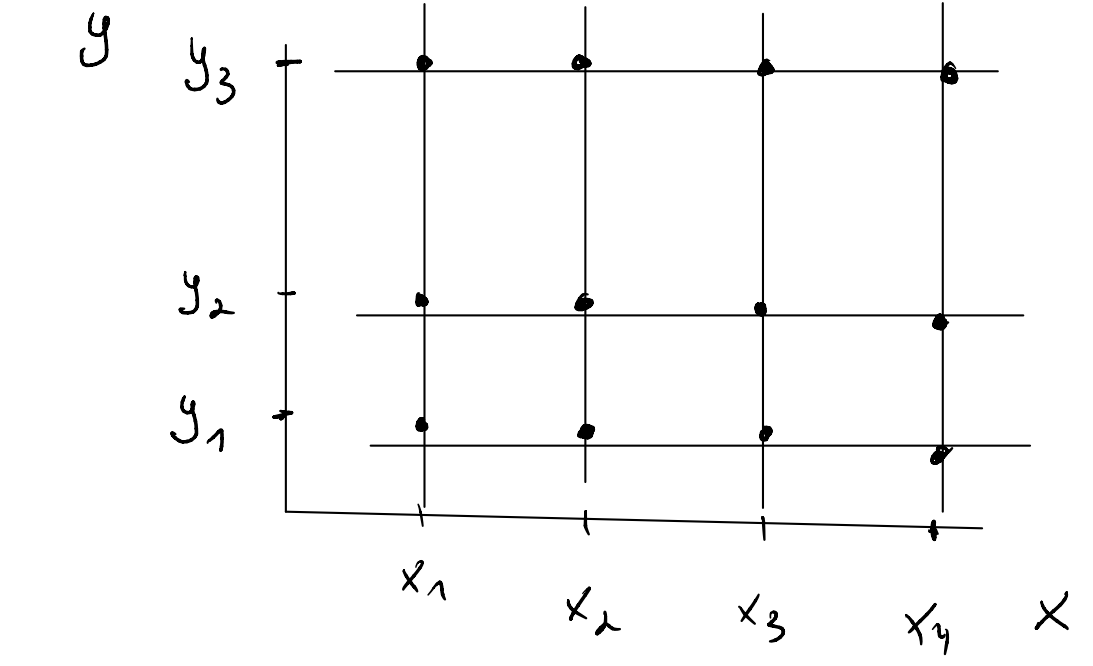
\includegraphics[scale=0.6]{../assets/multi_inter.png}
    \end{center}
    We are interpolating along the vertical and horizontal lines here.
\end{mdframed}
\textbf{Remark:} Points do not need to be equally spaced. In other words, it's not necessarily true that $y_2 - y_1 = y_1 - y_0$.

\subsubsection{Cardinal Functions}
Additionally, we only want to consider ``cardinal'' functions, i.e., functions $u_{i}(x)$ and $v_{j}(y)$ so that
\[u_{i}(x_{j}) = \delta_{i, j} = \begin{cases}
    1 & i = j \\ 
    0 & i \neq j
\end{cases}, \qquad v_{j}(x_{i}) = \delta_{j, i} = \begin{cases}
    1 & j = i \\ 
    0 & j \neq i
\end{cases}\]
for $1 \leq i, j \leq p$ and $1 \leq i, j \leq q$, respectively. We can construct such a cardinal function by 
\[u_{i}(x) = \prod_{\substack{j = 1 \\ j \neq i}}^{p} \frac{x - x_j}{x_i - x_j}\]
\[v_{j}(y) = \prod_{\substack{i = 1 \\ i \neq j}}^{q} \frac{y - y_i}{y_j - y_i}.\]
Let us define the set of vertical lines, 
\[L_{i} = \{(x_i, y) : -\infty < y < \infty\}.\]
Then, we can define the function \[(\bar{P}f)(x, y) = \sum_{i = 1}^{p} f(x, y) u_{i}(x) = P_{i}(x, y), \qquad P_{i}(x_{i}, y) = f(x_{i}, y).\]
Likewise, we have 
\[(\bar{Q}f)(x, y) = \sum_{j = 1}^{q} f(x, y_{j}) v_{j}(y).\]
There are two options for evaluating this: 
\begin{itemize}
    \item \underline{Option 1:} Consider the tensor product\footnote{Another way of writing this is $\bar{P} \otimes \bar{Q}$.}, 
    \[\bar{P}\bar{Q} = (\hat{P} (\bar{Q} f))(x, y) = \sum_{i = 1}^{p} \left( \sum_{j = 1}^{q} f(x_{i}, y_{j}) v_{j}(y) \right) u_{i}(x) = \sum_{i = 1}^{p} \sum_{j = 1}^{q} f(x_{i}, y_{i}) v_{j}(y) u_{i}(x) = F(x, y).\]
    This interpolates $f(x_{i}, y_{j}).$

    \item \underline{Option 2:} Consider the boolean sum. Then,  
    \begin{equation*}
        \begin{aligned}
            \bar{P} \oplus \bar{Q} &= \bar{P} + \bar{Q} - \bar{P}\bar{Q} \\
                &= \sum_{i = 1}^{p} f(x_{i}, y) u_{i}(x) + \sum_{j = 1}^{q} f(x, y_{j}) v_{j}(y) - \sum_{i = 1}^{p} \sum_{j = 1}^{q} f(x_{i}, y_{j}) v_{j}(y) u_{i}(x) \\ 
                    &= F(x, y).
        \end{aligned}
    \end{equation*}
    This is also an interpolation. 
\end{itemize}

\end{document}